\documentclass[12pt]{article}
\usepackage[dvipsnames]{xcolor}
\usepackage{hyperref, pagecolor, mdframed }
\usepackage{graphicx, amsmath, latexsym, amsfonts, amssymb, amsthm,
amscd, geometry, xspace, enumerate, mathtools}
\usepackage{tikz}

\theoremstyle{plain}
\newtheorem{thm}[subsubsection]{Th\'eor\`eme}
\newtheorem{lem}[subsubsection]{Lemme}
\newtheorem{prop}[subsubsection]{Proposition}
\newtheorem{propr}[subsubsection]{Propri\'et\'e}
\newtheorem{cor}[subsubsection]{Corollaire}
\newtheorem{intro}[section]{Introduction}
\newtheorem{thm2}[subsection]{Th\'eor\`eme}
\newtheorem{lem2}[subsection]{Lemme}
\newtheorem{prop2}[subsection]{Proposition}
\newtheorem{propr2}[subsection]{Propri\'et\'e}
\newtheorem{cor2}[subsection]{Corollaire}

\theoremstyle{definition}
\newtheorem{defn}[subsubsection]{D\'efinition}
\newtheorem{rmq}[subsubsection]{Remarque}
\newtheorem{conj}[subsubsection]{Conjecture}

\newtheorem{exmp}[subsubsection]{Exemples}
\newtheorem{quest}[subsubsection]{Exercices}
\newtheorem{defn2}[subsection]{D\'efinition}
\newtheorem{rmq2}[subsection]{Remarque}
\newtheorem{conj2}[subsection]{Conjecture}
\newtheorem{exmp2}[subsection]{Exemples}
\newtheorem{quest2}[subsection]{Exercices}

\theoremstyle{remark}
\newtheorem{rem}{Remarque}
\newtheorem{note}{Note}

\newcommand{\fdiv}{\textrm{div}}
\newcommand{\Z}{\mathbb{Z}}
\newcommand{\Q}{\mathbb{Q}}
\newcommand{\K}{\mathbb{K}}
\newcommand{\Proj}{\mathbb{P}}
\newcommand{\algK}{\overline{K}}
\newcommand{\algF}{\overline{\mathbb{F}}}
\newcommand{\Pic}{\textrm{Pic}}
\newcommand{\Hom}{\textrm{Hom}}
\newcommand{\End}{\textrm{End}}
\newcommand{\C}{\mathbb{C}}
\newcommand{\w}{\omega}
\newcommand{\h}{\mathfrak{h}}
\newcommand{\La}{\mathcal{L}}
\newcommand{\F}{\mathcal{F}}
\hypersetup{
    colorlinks=true,
    linkcolor=blue,
    urlcolor=Green,
    filecolor=RoyalPurple
}

\definecolor{wgrey}{RGB}{148, 38, 55}
\title{Modular forms}
\date{13 aout 2023}
\begin{document}
\maketitle
\tableofcontents

\section{formes modulaires}
 
\subsection{Le formalisme}
D'abord les objets : on va considérer 
\begin{itemize}
    \item $SL_2(\Z)$ le groupe spécial linéaire.
    \item $\h:=\{\tau\in\C\mid Im(\tau)>0\}$ le demi plan de poincaré.
    \item $\h/SL_2(\Z)$ le quotient de $\h$ par l'action de $SL_2(\Z)$.
\end{itemize}

Ensuite les morphismes :
\begin{itemize}
    \item Avec $\La :=\{\Lambda\mid \Lambda\text{ est un reseau sur }\C\}$ : $$\La/\C^*\approx \text{SL}_2(\Z)\backslash\h$$
    \item Et : $$\La/\C^*\approx \frac{\{\text{elliptic curves over }\C\}}{\C-\text{isomorphism}}$$
\end{itemize}
La deuxième fleche est injective et bijective via le théorème \textbf{d'uniformisation}.
\newpage

Comme $\pm I$ agit trivialement sur un réseau, on considère en fait :
\begin{defn}
    On définit $\Gamma(1) = \text{SL}_2(\Z)/\{\pm 1\}$.
\end{defn}

\begin{rem}
    On définit $S=\begin{pmatrix} 0 & -1\\ 1 & 0\\ \end{pmatrix}$ et $T=\begin{pmatrix} 1 & 1\\ 0 & 1\\ \end{pmatrix}$. Alors on verra que
    $\Gamma(1)=<S,T>$. En plus $S$ est d'ordre $2$ et $ST$ d'ordre $3$. L'action est donnée par :
    \begin{itemize}
        \item $S(\tau)=-1/\tau$ et $T(\tau)=\tau+1$.
    \end{itemize}
\end{rem}

Le domaine fondamental :
\begin{prop}
    $\F:=\{\tau\in\h:\lvert\tau\rvert\geq1 \text{ et } \lvert\text{Re}(\tau)\rvert\leq 1/2\}$ définit un bon domaine fondamental
    au sens ou $\gamma\tau,\tau\in\F$ implique que 
    \begin{itemize}
        \item Re$(\tau)=\pm1/2$(chelou).
        \item $\lvert\tau\rvert=1$.

    \end{itemize}
    Et pour tout $\tau$ il existe $\gamma$ tq $\gamma\tau\in\F$. En plus les stabilisateurs sont triviaux SAUF pour :
    \begin{itemize}
        \item i, $\rho=e^{2i\pi/3}$, $-\overline{\rho}$.
    \end{itemize}
\end{prop}
\begin{cor}
    $\Gamma(1)=<S,T>$. 
\end{cor}
Ca tombe direct psq pour $\gamma\in <S,T>$ : il existe $\gamma'\in <S,T>$ tq $\gamma'(\gamma\tau)\in\F$. En prenant
un élément de stabilisateur trivial on a fini.


\subsubsection{Remarques sur la preuve}
Deux points :
\begin{itemize}
    \item $T^n\tau=\tau+n$ d'ou on peut supp Re$(\tau)\leq1/2$.
    \item Im$(\gamma\tau)=\frac{\text{Im}(\tau)}{\lvert c\tau+d\rvert^2}$ et $\lvert c\tau+d\rvert^2=(cs+d)^2+(ct)^2$ d'ou 
le module croit vers $\infty$ avec $c, d$. On peut donc minimiser Im$(\gamma\tau)$. D'ou si $\lvert\tau\rvert<1$ comme 
$$\text{Im}(S\gamma\tau)=\frac{\text{Im}(\tau)}{\lvert\gamma\tau\rvert^2}>\text{Im}\gamma\tau$$
On a une contradiction.
\end{itemize}

\subsection{La courbe modulaire}
En regardant $\F$, on remarque que les deux droites verticales sont identifiées par $T$ et les deux arcs de l'arc
formant le côté borné de $\F$ sont identifié par $S$. D'ou en recollant On obtient une $2$-sphere privée d'un point !\\
On rajoute des points pour en faire une surface de Riemann intéressante :

\begin{defn}
    On définit $\h^*=\h\cup\Proj^1(\Q)=\h\cup\Q\cup\{\infty\}$. Ou les points de $\Proj^1(\Q)$ sont les \textbf{pointes}.(cusps)
    Et on étend l'action de $\Gamma(1)$ à $\h^*$ via :
    \begin{itemize}
        \item $\begin{pmatrix} a&b\\c&d\\ \end{pmatrix}[x,y]=[ax+by,cx+dy]$. (par homographie)
    \end{itemize}
\end{defn}

Puis on définit :
\begin{defn}
    $Y(1)=\Gamma(1)\backslash\h$ et $X(1)=\Gamma\backslash\h^*$. 
\end{defn}
\begin{rem}
    En fait, $X(1)$ a une seule pointe : $\infty$. On prend $[x,y]$ tq $ax+by=1$, 
    alors
    \begin{itemize}
        \item $\begin{pmatrix}a&b\\ -y & x\\ \end{pmatrix}[x,y]=[1,0]=\infty$.
    \end{itemize}
\end{rem}

\subsection{La topologie de X(1)}
On veut une topologie qui ressemble à une $2$-sphere.
\begin{defn}
    On prend comme base de la topologie :
    \begin{itemize}
        \item Sur $\h$ les ouverts de $\C$.
        \item Pour $\infty$ les ensembles du type $\{\text{Im}(\tau)>\kappa\}\cup\{\infty\}$ pour tout $\kappa$.
        \item Pour les autres pointes les boules ouvertes tangentes à l'axe réel contenues dans $\h$ + la pointe : $B(a, r)\cup \{\tau\}$
    \end{itemize}
\end{defn}

\begin{rem}
    La topologie est Hausdorff (clair) et l'action est transitive sur les ouverts des pointes.
\end{rem}

\newpage
Maintenant un lemme important : 
\begin{defn}
    On définit
    \begin{itemize}
        \item $\forall\tau_1,\tau_2$ on def $I(\tau_1,\tau_2)=\{\gamma : \gamma\tau_1=\tau_2\}$.
        \item $\forall U_1,U_2$ on def $I(U_1,U_2)=\{\gamma : \gamma U_1\cap U_2\ne\emptyset\}$.
    \end{itemize}
\end{defn}
\begin{lem}
    Pour tout $\tau_1,\tau_2$ il existe $U_1,U_2$ tq $$I(U_1,U_2)=I(\tau_1,\tau_2)$$
    En particulier si on peut rendre $U_1,U_2$ suffisamment petits alors $\tau_1=\gamma \tau_2$.
\end{lem}
\textbf{Preuve :} Le cas (nombre, nombre) : la preuve consiste à remarquer que $I(\F,\F)$ est fini d'ou si $G=\text{Interior}\left(\cup_{\gamma\in I(\F,\F)}\quad \gamma\F\right)$,
$I(G,G)$ aussi. \\ \indent On prend $\gamma\in I(G,G)\backslash I(\tau_1,\tau2)$ et des ouverts $V_{\gamma}, W_{\gamma}$ qui les séparent. 
Puis $$U_1=G\cap \bigcap_{\gamma\in I(G,G)\backslash I(\tau_1,\tau_2)} \gamma V_{\gamma}$$ et $$U_2=G\cap \bigcap_{\gamma\in I(G,G)\backslash I(\tau_1,\tau_2)} \gamma W_{\gamma}$$
Alors $I(\tau_1,\tau_2)\subseteq I(U_1,U_2)$, l'égalité se montre par contradiction. Quand $\tau_1=\tau_2$ sont la pointe on a $I(\infty,\infty)=I(\{\text{Im}(\tau)>2\},\{\text{Im}(\tau)>2\})=\{T^k:k\}$.\\
\indent Dans le cas (pointe,nombre) $I(pointe,nombre)=\emptyset$!\qed

\begin{rem}
    Le $G$ est le gros contour du dessin usuel et $I(\F,\F)$ est fini via le dessin aussi.
\end{rem}

On prend définit
\begin{defn}
    La topologie de $X(1)$ comme la topologie quotient donnée par 
    \begin{align*}
        \phi : \h^*\rightarrow \Gamma(1)\backslash \h^*=X(1)
    \end{align*}
\end{defn}

\noindent Alors 
\begin{prop}
    $X(1)$ est compacte Hausdorff.
\end{prop}

\begin{rem}
    L'idée pour la compacité est de remarquer que d'un ouvert contenant $\infty$, $\phi^{-1}(\infty)$ contient un ouvert non borné, en fait LE ouvert non borné.
    Hausdorff c'est clair.
\end{rem}

\newpage

\subsection{La structure de surface de Riemann}
Celle la va être longue mais nécessaire.\\

On prend la structure suivante : 
\begin{defn}
    Le recouvrement : pour chaque $\phi(\tau_x)=x\in X(1)$ il existe $U_x$ tq $I(U_x,U_x)=I(\tau_x)$ alors on
prend $I(\tau_x)\backslash U_x$ comme voisinage de $x$.\\
\newline
\indent Les homéomorphismes :
    \begin{itemize}
        \item Pour $x\in X(1)\backslash\{\infty\}$ tel que $\# I(\tau_x)=r$: On définit 
        \begin{align*}
            \psi_x~:~I(\tau_x)\backslash U_x&\rightarrow \C\\
                \phi(\tau)&\mapsto \left(\frac{\tau-\tau_x}{\tau-\overline{\tau_x}}\right)^r\\
        \end{align*}
        \item Pour $x=\infty$ on prend $\tau_x=\infty$ d'ou $I(\tau_x)=\{T^k\}$ et on pose:
        \begin{align*}
            \psi_x~:~I(\tau_x)\backslash U_x\rightarrow& \C\\
                \phi(\tau)\mapsto& ~e^{2\pi i\tau}\text{  si } \phi(\tau)\ne \infty\\
                                 & ~0 ~~\quad \text{ si } \phi(\tau)=\infty\\
        \end{align*}
    \end{itemize}
\end{defn}

\newpage
On a les deux diagrammes :\\ 
\begin{itemize}
    \item Pour $x\ne\infty$
\end{itemize}

\begin{center}
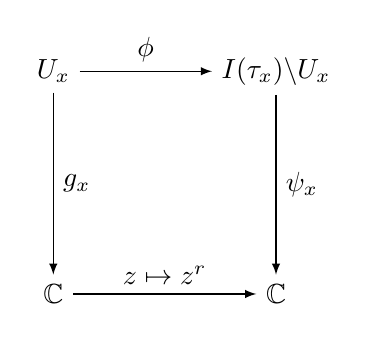
\begin{tikzpicture}[x=1cm,y=1cm, >=latex, ->]
    \node(0) at (135 : 2) {$U_x$};
    \node(1) at (45 : 2) {$ I(\tau_x)\backslash U_x$};
    \node(2) at (-135 : 2) {$\C$};
    \node(3) at (-45 : 2) {$\C$};

    \draw(0)--(1) node[midway, above]{$\phi$};
    \draw(1)--(3) node[midway, right]{$\psi_x$};
    \draw(2)--(3) node[midway, above]{$z\mapsto z^r$};
    \draw(0)--(2) node[midway, right]{$g_x$};
\end{tikzpicture}
\end{center}

\begin{itemize}
    \item Pour $x=\infty$ :
\end{itemize}

\begin{center}
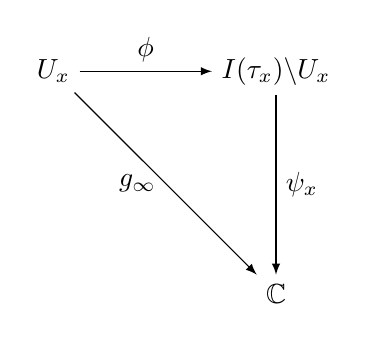
\begin{tikzpicture}[x=1cm,y=1cm, >=latex, ->]
    \node(0) at (135 : 2) {$U_x$};
    \node(1) at (45 : 2) {$ I(\tau_x)\backslash U_x$};
    \node(2) at (-45 : 2) {$\C$};

    \draw(0)--(1) node[midway, above]{$\phi$};
    \draw(1)--(2) node[midway, right]{$\psi_x$};
    \draw(0)--(2) node[midway, left]{$g_{\infty}$};
\end{tikzpicture}
\end{center}
\newpage

\begin{itemize}
    \item Pourquoi ca marche ? 
\end{itemize}

Les étapes, d'abord les $\psi_x$ sont des homéomorphismes :

\begin{enumerate}
    \item $I(\tau_x)$ est cyclique engendré par $\gamma$.
    \item $g_x\circ\gamma\circ g_x^{-1}(z)$ est un conjugué d'homographies ayant pour points fixes $0,\infty$.
    \item D'ou $G(z)=g_x\circ\gamma\circ g_x^{-1}(z)=cz$ (voir wiki) puis $G\circ...\circ G(z)=z$ d'ou $$g_x(\gamma \tau)=\zeta_rg_x(\tau)$$.
    \item alors $\psi_x$ est bien définie et clairement continue, ouverte.
    \item l'injectivé est assez claire faut bien écrire les defs.
\end{enumerate}

\noindent Les changements de cartes sont biholomorphes :
\begin{enumerate}
    \item L'idée est que pour $x,y\in X(1)\backslash \{\infty\}$ on écrit :$$\phi_y\circ\phi_x^{-1}(z)=g_y^{r_y}\circ g_x^{-1}(z^{1/r_x})$$
    \item Le problème vient de la puissance inverse. Mais $$\phi_y\circ\phi_x^{-1}(\zeta_{r_x}z)=g_y^{r_y}\circ g_x^{-1}(z)$$
    \item On en déduit en comparant les séries entières que on a une série entière en $z^{r_x}$. D'ou la biholomorphie.
    \item Pour $x,\infty$ c'est le même genre d'idée avec un log.
\end{enumerate}
\newpage


\subsection{fonctions modulaires}
L'intuition des definitions viendra plus tard. (formes différentielles sur la courbe modulaire)
\begin{defn}
    Faible modularité de poids $2k$ de $f$ :
    \begin{itemize}
        \item Méromorphie sur $\h$
        \item $f(\gamma\tau)=(c\tau+d)^{2k}f(\tau)$ pour tout $\gamma$ dans $\Gamma(1)$.
    \end{itemize}
\end{defn}

\begin{rem}
    En fait il suffit que :
    \begin{itemize}
        \item $f(\tau+1)=f(\tau)$
        \item $f(-1/\tau)=\tau^{-2k}f(\tau)$
    \end{itemize}
    
\end{rem}

\begin{rem}
    Ducoup la periodicité fournit un développement de fourier en $q=e^{2i\pi\tau}$, $\overline{f}(q)=\sum_{n=-\infty}^{+\infty}a_nq^n$. 
\end{rem}
\begin{defn}
    $f$ est :
    \begin{itemize}
        \item meromorphe à l'infini si y'a un $n=n_0$ minimal tq $a_n=0$ pour $n<n_0$.
        \item holomorphe à l'infini si $n_0=0$.
    \end{itemize}
    Quand $f$ est méromorphe à l'infini son ordre est donné par  :
    \begin{itemize}
        \item $ord_{\infty}(f)=-n_0$
    \end{itemize}
    Quand $f$ est holomorphe à l'infini on peut l'évaluer via :
    \begin{itemize}
        \item $f(\infty)=\overline{f}(0)=a_0$
    \end{itemize}
\end{defn}

\begin{defn}
    Une fonction 
    \begin{itemize}
        \item faiblement modulaire
        \item meromorphe à l'$\infty$
    \end{itemize}
    est appelée une fonction modulaire. Si en plus elle est 
    \begin{itemize}
        \item holomorphe à l'$\infty$
    \end{itemize}
    alors on l'appelle une \textbf{forme modulaire}. Enfin si en plus
    \begin{itemize}
        \item $f(\infty)=0$
    \end{itemize}
    on dit que la forme est \textbf{cuspidale}.
\end{defn}

\subsubsection{Les formes Eisenstein}
Les séries d'Eisenstein, $G_{2k}(\Lambda):=\sum_{\w\in\Lambda^*}\frac{1}{(\w)^{2k}}$ (ou $G_{2k}(\tau)=G_{2k}([1,\tau])$), sont un type important de formes modulaires. Pour le voir : (on note $\rho=e^{2i\pi/3}$)
\begin{enumerate}
    \item C'est clair que $G_{2k}(c\Lambda)=c^{-2k}G_{2k}(\Lambda)$ d'ou $G_2k(\gamma\tau)=G_{2k}((c\tau+d)^{-1}[1,\tau])=(c\tau+d)^{2k}G_{2k}(\tau)$
    \item Sur $\F$, on a $$\lvert m\tau+n\rvert^2\geq m^2-mn+n^2=\lvert m\rho-n\rvert^2$$ d'ou une majoration uniforme et l'holomorphie sur $\F$
L'holomorphie suit via la modularité qui lie les translatés de $\F$.
    \item Quand $\tau\rightarrow i\infty$, les termes ou $m\ne0$ tendent vers $0$ d'ou $$\lim_{\tau\rightarrow i\infty}G_{2k}(\tau)=2\zeta(2k)$$ et l'holomorphie à l'$\infty$.
\end{enumerate}

\begin{rem}
    On pose $g_2(\tau)=60G_4(\tau)$ et $g_3(\tau)=140G_6(\tau)$.\\
    \indent On voit facilement que $\Delta=g_2^3-27g_3^2$ est une forme modulaire de poids $12$.
    Via la formule pour $G_{2k}(\infty)$ et les valeurs connnues de 
    \begin{align*}
        &\zeta(4)=\frac{\pi^4}{90} &\zeta(6)=\frac{\pi^6}{945}\\
    \end{align*} 
    on obtient $\Delta(\infty)=0$. D'ou $\Delta$ est une forme cuspidale de poids $12$.
\end{rem}


\subsection{k-formes différentielles et formes modulaires}
D'abord sur $X/\C$ une courbe projective lisse :
\begin{defn}
    On note $$\Gamma_{X}^k=\Gamma_X\otimes_{C(X)}...\otimes_{C(X)}\Gamma_X$$ L'espace des $k$-formes différentielles ou $\Gamma_X$ est l'espace
    des $1$-formes.
\end{defn}
Bon la je crois que vu qu'on prend pas le produit exterieur c'est de dim $1$.
\begin{defn}
    Pour $\w\in\Gamma_X^k$ et $t$ d'ordre $1$ en $x\in X$ on a $$\w=g(dt)^k$$
    on def $$ord_x(\w)=ord_x(g)$$
    et $$div(\w)=\sum_{x\in X}ord_x(\w)(x)\in Div(X)$$
\end{defn}

\begin{prop}
    On supp que $X$ est de genre $g$.\begin{enumerate}
        \item $div(\w)\sim kK_X$. ($div(\w)=kdiv(\eta)+div(\w/\eta^k)$ et $\w/eta^k\in \C(X)$)
        \item $deg(div(\w))=k(2g-2)$. (Riemann-Roch)
    \end{enumerate}
\end{prop}

Le lien entre les différentielles et les forme modulaire et comportement local de $\w_f$.
\begin{prop}
    $f$ une fonction modulaire de poids $2k$.
    \begin{enumerate}
        \item Il existe $\w_f\in\Gamma_{X(1)}^k$ tq $\phi^*(\w_f)=f(\tau)(d\tau)^k$.
        \item $ord_x(\w_f)=\begin{cases}
            ord_{\tau_x}(f) &if~x\ne\phi(i),\phi(\rho),\phi(\infty);\\
            \frac{1}{2}ord_i(f)-\frac{1}{2}k &if~ x=\phi(i);\\
            \frac{1}{3}ord_{\rho}(f)-\frac{2}{3}k &if~x=\phi(\rho);\\
            ord_{\infty}(f)-k &if~x=\phi(\infty).
        \end{cases}$
    \end{enumerate}
\end{prop}
La preuve est un peu longue j'essaie de résumer les étapes.
\begin{rem} A noter avant :
    \begin{enumerate}
        \item $(d\gamma\tau)^k=(c\tau+d)^{-k}(d\tau)^k$ d'ou $f(\tau)(d\tau)^k$ est $\Gamma(1)$-invariante !
        \item Si $z=g_x(\tau)=\frac{\tau-\tau_x}{\tau-\overline{\tau_x}}$ alors 
        \begin{align*}
            g_x(R\tau)&=\zeta g_x(\tau)\\
            \leftrightarrow R\tau&=g_x^{-1}(\zeta z)=g_x^{-1}(\zeta z)\\
        \end{align*}
    \end{enumerate}
\end{rem}

\textbf{Etapes de la preuve :} D'abord $x\ne\infty$ \begin{enumerate}
    \item $f(\tau)(d\tau)^k=f(g_x^{-1}(z))((g_x^{-1})')^k(dz)^k=F(z)(dz)^k$
    \item $F(z)(dz)^k=f(\tau)(d\tau)^k=f(R\tau)(dR\tau)^k=F(\zeta z)(d\zeta z)^k=F(\zeta z)\zeta^k(dz)^k$
    \item D'ou $F(z)z^k$ est invariante par $z\mapsto \zeta z$ puis $F(z)z^k=F_1(z^r)$.
    \item Enfin on peut réecrire, en posant $w=z^r$, $F(z)(dz)^k=r^{-k}z^{k(1-r)}F(z)(dz^r)^k=r^{-k}w^{-k}F_1(w)(dw)^k$
\end{enumerate}
Et le calcul des ordres est direct on obtient :
\begin{itemize}
    \item $ord_x\w_f=\frac{1}{r}ord_{\tau_x}f-(1-\frac{1}{r})k$
    \item ou via le cardinal des stabilisateurs $r=1,2\text{ ou }3$
\end{itemize}
Le calcul pour $x=\infty$ est aussi direct.\qed

Le comportement global de $\w_k$ est donné par le
\begin{cor}
    $f$ une fonction modulaire de poids $2k$. Alors
    \begin{itemize}
        \item $\frac{1}{2}ord_i(f)+\frac{1}{3}ord_{\rho}+ord_{\infty}(f)+\sum_{autres~\tau}ord_{\tau}(f)=\frac{k}{6}$
    \end{itemize}
\end{cor}
\textbf{Idée :} Simple conséquence de la prop précedente et du fait que $$deg(div(\w_f))=-2k$$.\qed

On pourra mtn donner de bonne description des espaces de forme modulaires d'un poids donné. 
\begin{defn}On pose :
    \begin{itemize}
        \item $M_{2k}=\{\text{formes modulaires de poids 2k pour }\Gamma(1)\}$
        \item $M_{2k}^{0}=\{\text{formes cuspidales de poids 2k pour }\Gamma(1)\}$
    \end{itemize}
\end{defn}

\begin{rem}
    $M=\bigoplus_{k=0}^{\infty}M_{2k}$ est un anneau gradué intègre. 
\end{rem}

\begin{thm}
    On a  :
    \begin{enumerate}
        \item $M_{2k}\cong M_{2k}^0\bigoplus\C G_{2k}$ via \begin{align*}
            M_{2k}&\rightarrow \C\\
            f&\mapsto f(\infty)
        \end{align*}
        \item $M_{2k}\cong M_{2k+12}^0$ via $f\mapsto f\Delta$. (facile)
        \item $dim(M_{2k})=\begin{cases}
            [k/6] &if~k\equiv 1~mod~6\\
            [k/6]+1 &if~k\neq  1~mod~6
        \end{cases}$, Ca se prouve en calculant les $6$ premiers $k$ et par recurrence.
    \end{enumerate}
\end{thm}

\section{q-expansions de courbes elliptiques et formes modulaires}
\subsection{Des fonctions quasi elliptiques}
On remarque que $\wp$ n'a pas de résidu on peut l'intégrer terme à terme et ajuster à chaque fois la constante
pour avoir la convergence.
\begin{defn}
    Fonction $\zeta$ de Weierstrass : $$\zeta(z;\Lambda):=\frac{1}{z}+\sum_{\w\in\Lambda^*}\left(\frac{1}{z-\w}
    +\frac{1}{\w}+\frac{z}{\w^2}\right)$$
    Et son développement en $0$ :$$\zeta(z;\Lambda)=\frac{1}{z}-\sum_{k=1}^{\infty}G_{2k+2}z^{2k+1}$$
\end{defn}

A remarquer que $\zeta'=-\rho$ en $z$ et ducoup la dérivée est périodique. On regarde l'implication
de $(\zeta(z+w; \Lambda)-\zeta(z;\Lambda))'=0$ sur $\zeta$.

\begin{prop}
    On def $\eta(\w)=\zeta(z+\w)-\zeta(z)$ (la quasi-periode) alors \begin{enumerate}
        \item $\eta$ est un homomorphisme (clair)
        \item si $\w$ est pas dans $2\Lambda$ (d'ou $\frac{w}{2}$ est pas un pole pour $\zeta$) :$$\eta(\w)=2\zeta(\frac{w}{2};\Lambda)$$
        \item Si $\Lambda=[\w_1,\w_2]$ tq $\frac{\w_1}{\w_2}>0$ alors $$\w_1\eta(\w_2)-\w_2\eta(\w_1)=2\pi i$$C'est la relation de Legendre. (résidu autour de $0$)
    \end{enumerate}
\end{prop}
Y s'avère que si on écrit $E:=E_{\Lambda}$ alors $\wp(z;\Lambda)dz=x\w_E$ et $\gamma\mapsto\int_{\gamma}x\w_E$
Fournit un autre morphisme $H^1(E(\C),\Z)\rightarrow \C$ donné par 

Fonction $\sigma$ :




\end{document}
